\begin{figure}[!htbp]
	\begin{subfigure}{\linewidth}
		\centering
		\begin{tabular}{>{\centering}p{3cm}c}
			\(
			\begin{bmatrix}
				\cos(\theta) & -\sin(\theta) & t_x \\
				\sin(\theta) & \cos(\theta)  & t_y \\
				0            & 0             & 1   \\
			\end{bmatrix}
			\)
			 &
			\(
			\vcenter{
				\hbox{
					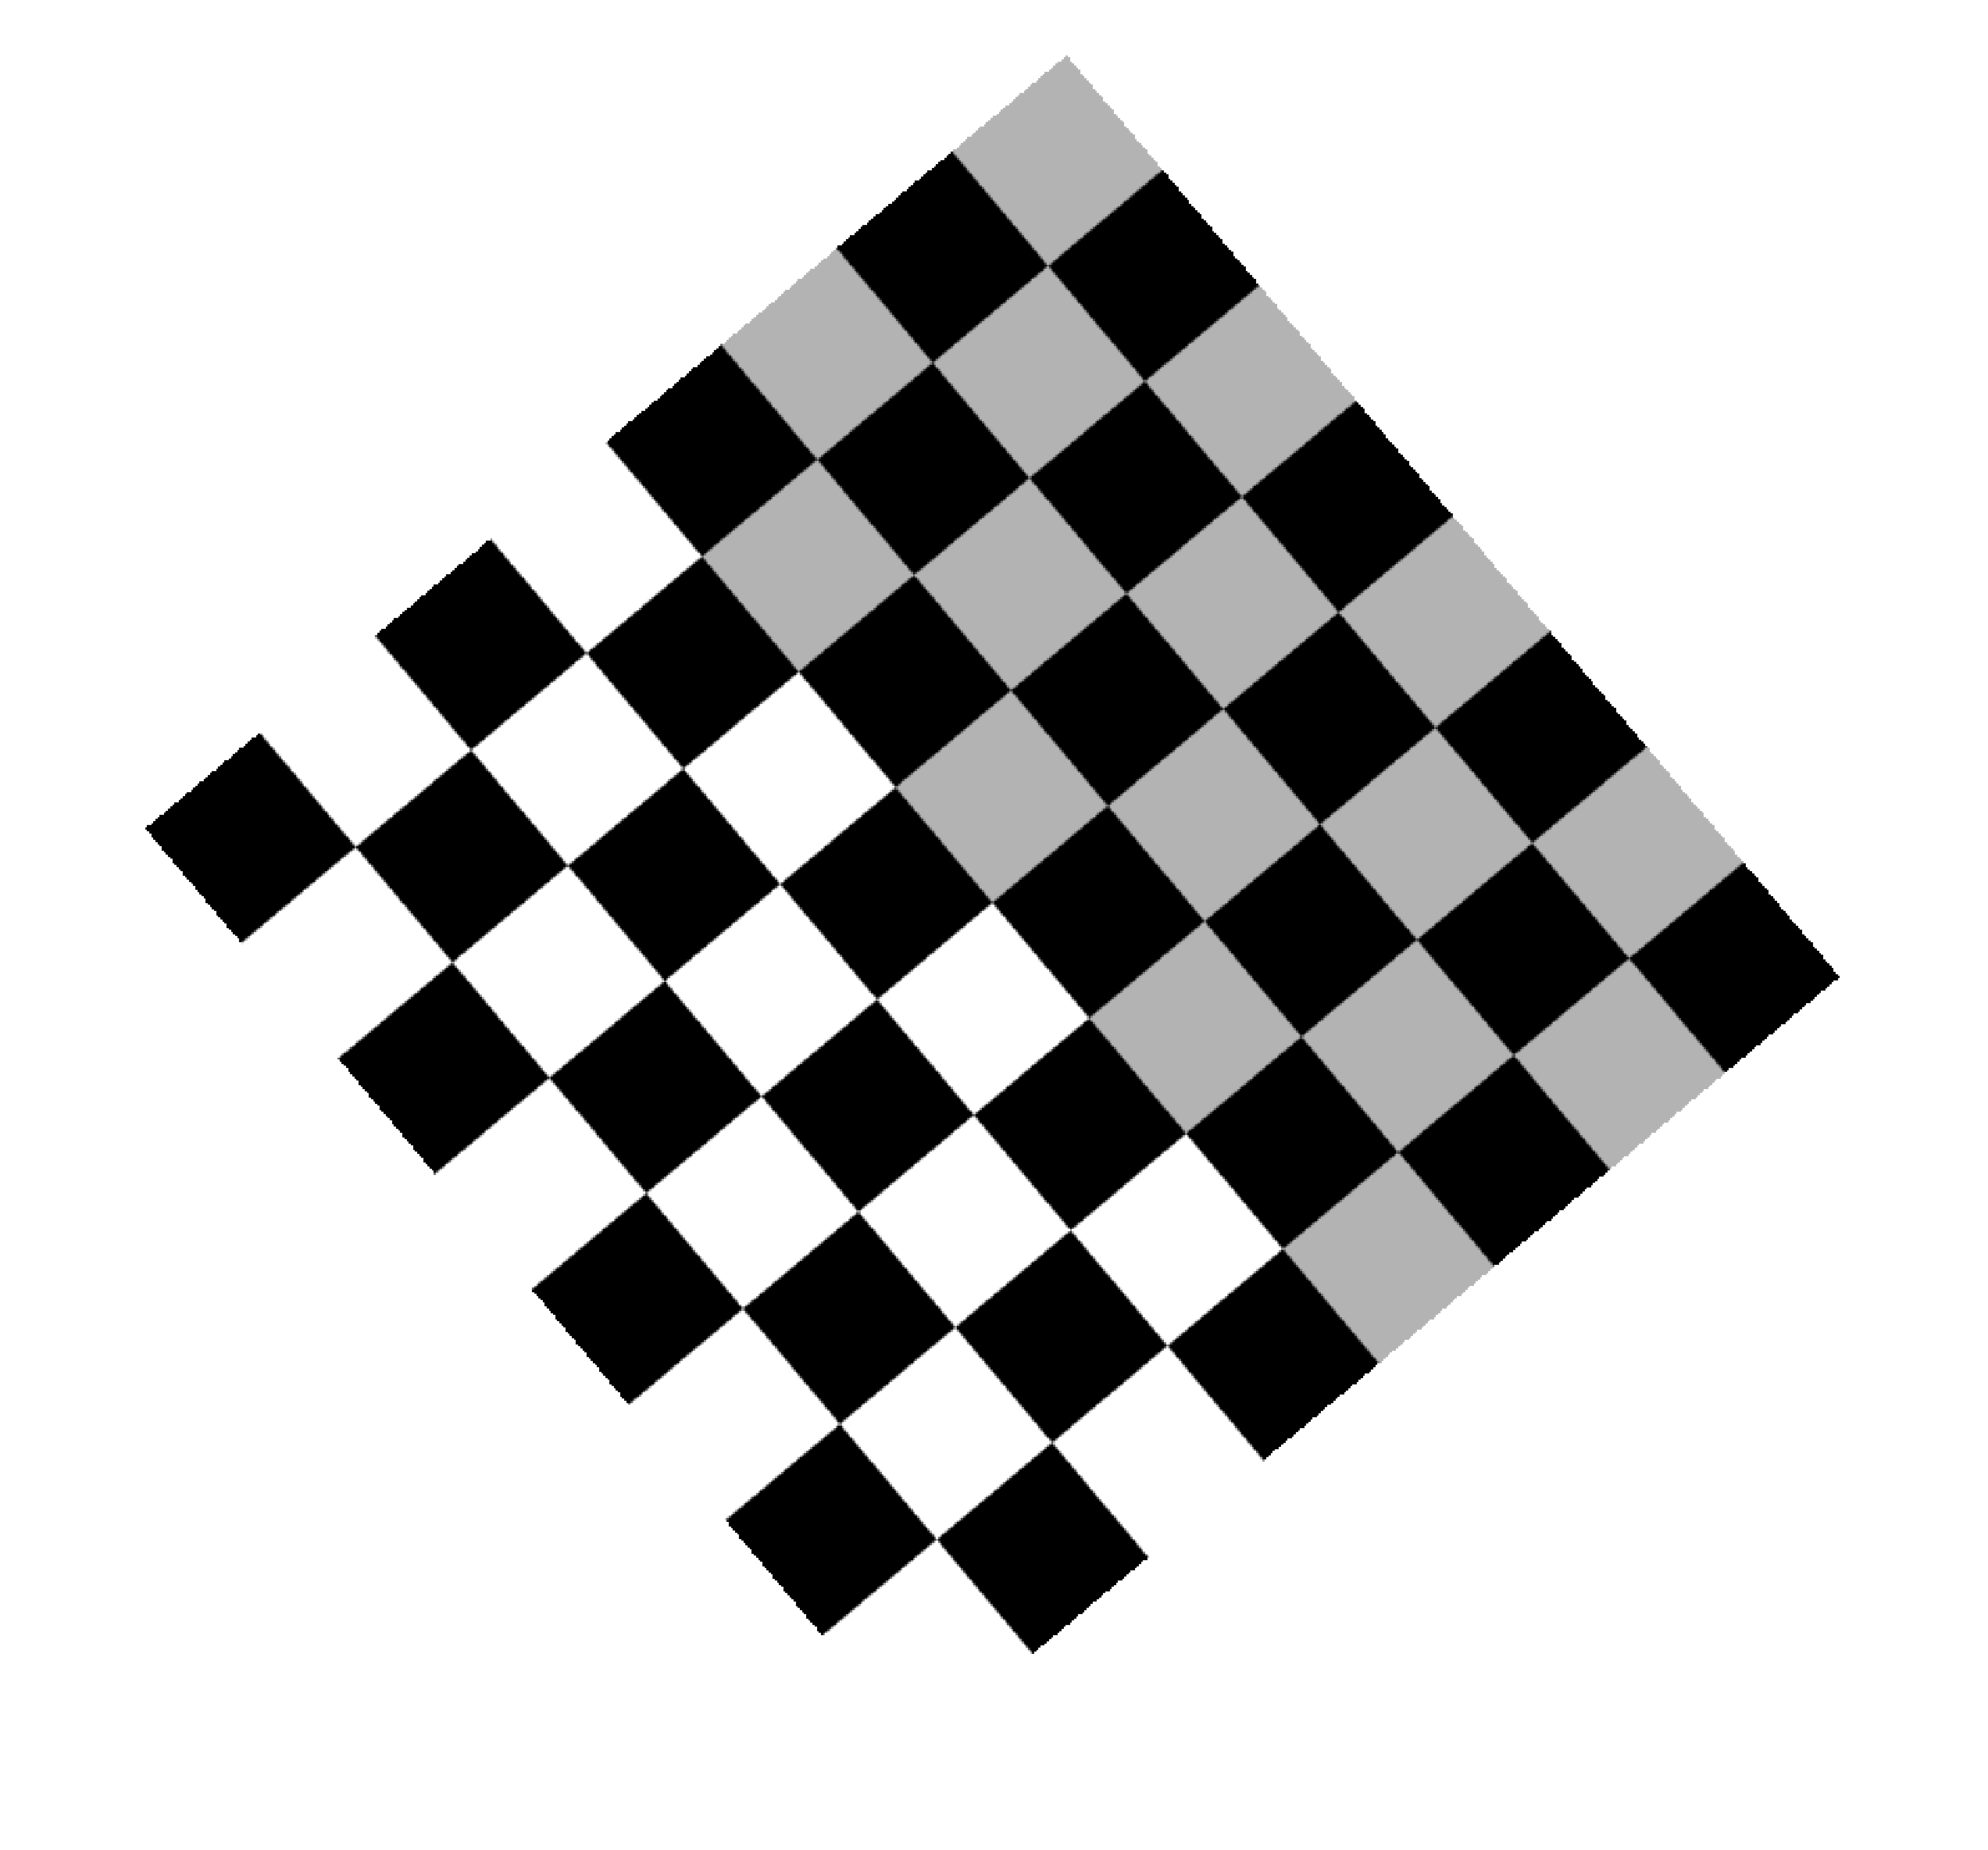
\includegraphics[height=.5\linewidth,width=.5\linewidth]{figures/registration/transforms/similarity.png}
				}
			}
			\)
		\end{tabular}
		\caption{Rigid transformation (isometry), i.e.,a rotation by \(\theta\) and translation by \((t_x, t_y)\).} \label{fig:rigidtransformation}
	\end{subfigure}
	\begin{subfigure}{\linewidth}
		\centering
		\begin{tabular}{>{\centering}p{3cm}c}
			\(
			\begin{bmatrix}
				a & b & t_x \\
				c & d & t_y \\
				0 & 0 & 1   \\
			\end{bmatrix}
			\)
			 &
			\(
			\vcenter{
				\hbox{
					
\includegraphics[height=.5\linewidth,width=.5\linewidth]{figures/registration/transforms/affine.png}
				}
			}
			\)
		\end{tabular}
		\caption{Affine transformation, i.e.,arbitrary transformations in the plane (including shear).} \label{fig:affinetransformation}
	\end{subfigure}
	\begin{subfigure}{\linewidth}
		\centering
		\begin{tabular}{>{\centering}p{3cm}c}
			\(
			\begin{bmatrix}
				a & b & c \\
				d & e & f \\
				g & h & i \\
			\end{bmatrix}
			\)
			 &
			\(
			\vcenter{
				\hbox{
					
\includegraphics[height=.5\linewidth,width=.5\linewidth]{figures/registration/transforms/projective.png}
				}
			}
			\)
		\end{tabular}
		\caption{Projective (perspective) transformation (homography).} \label{fig:projectivetransformation}
	\end{subfigure}
	\begin{subfigure}{\linewidth}
		\centering
		\begin{tabular}{>{\centering}p{4cm}c}
			\(
			\begin{bmatrix}
				a(x,y) & b(x,y) & c(x,y) \\
				d(x,y) & e(x,y) & f(x,y) \\
				g(x,y) & h(x,y) & i(x,y) \\
			\end{bmatrix}
			\)
			 &
			\(
			\vcenter{
				\hbox{
					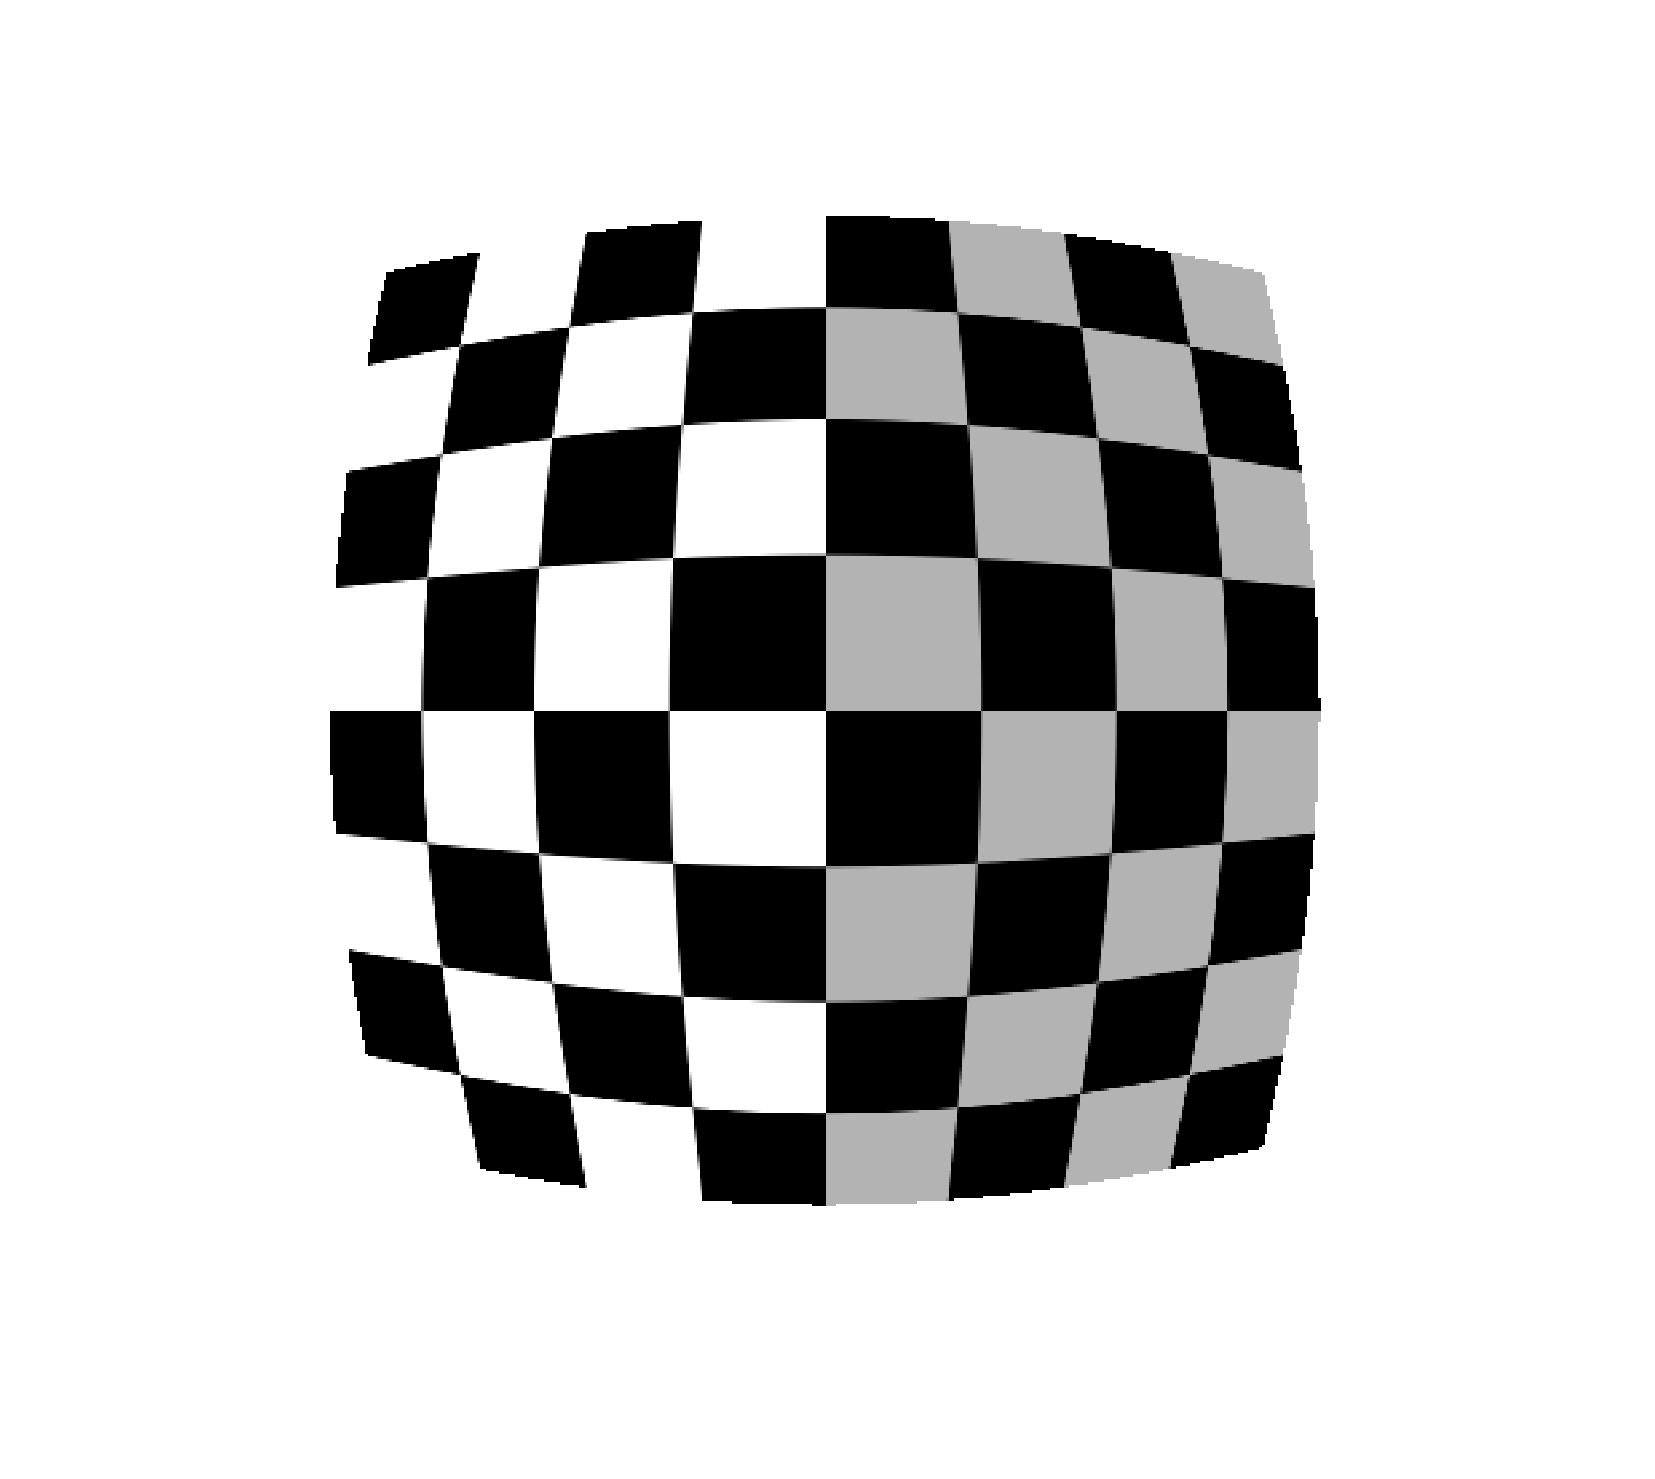
\includegraphics[height=.5\linewidth,width=.5\linewidth]{figures/registration/transforms/barrel.png}
				}
			}
			\)
		\end{tabular}
		\caption{Elastic transformation, i.e.,locally defined transformation.} \label{fig:elastictransformation}
	\end{subfigure}
	\caption[Compact Routing Example]{Different transformation classes (in homogeneous coordinates) along with realized examples.}
	\label{fig:transformations}
\end{figure}
